% Compute-Aware MoE for 5G Neural Receivers — KNN poster
% A1 portrait, tikzposter
% Build: pdflatex poster.tex

\documentclass[a1paper,portrait,25pt,margin=15mm,innermargin=12mm,colspace=15mm,blockverticalspace=12mm,subcolspace=8mm]{tikzposter}

\usepackage[utf8]{inputenc}
\usepackage[T1]{fontenc}
\usepackage{lmodern}
\usepackage{graphicx}
\usepackage{booktabs}
\usepackage{array}
\usepackage{amsmath}

\usetheme{Simple}
\usetitlestyle{Empty}
\useblockstyle{Default}

% Wong color-blind safe palette to match the figures.
% Deep blue for headers (matches dense_large in plots), vermilion for the hero accent.
\definecolor{deepblue}{RGB}{0,61,96}
\definecolor{lightbg}{RGB}{246,248,250}
\definecolor{accent}{RGB}{213,94,0}
\definecolor{darkgray}{RGB}{50,50,50}
\definecolor{fitteal}{RGB}{0,61,96} % alias kept so existing \color{fitteal} still works

\definecolorstyle{wong}{}{
  \colorlet{titlebgcolor}{deepblue}
  \colorlet{titlefgcolor}{white}
  \colorlet{blocktitlebgcolor}{deepblue}
  \colorlet{blocktitlefgcolor}{white}
  \colorlet{blockbodybgcolor}{white}
  \colorlet{blockbodyfgcolor}{darkgray}
  \colorlet{backgroundcolor}{lightbg}
  \colorlet{framecolor}{deepblue}
  \colorlet{notebgcolor}{accent}
  \colorlet{notefgcolor}{white}
}
\usecolorstyle{wong}

% Disable the tikzposter watermark
\tikzposterlatexaffectionproofoff

\title{\parbox{\linewidth}{\centering Compute-Aware Mixture-of-Experts \\[0.2em] for Efficient 5G Neural Receivers}}
\author{Dominik Huml \quad Jakub Kontrik \quad Martin Vaculik}
\institute{Faculty of Information Technology, Brno University of Technology \\ KNN course project, 2026}

\begin{document}

\maketitle[width=\textwidth]

%==============================================================================
% HERO BAND: Headline result
%==============================================================================
\block{The headline result}{
  \begin{minipage}{0.55\linewidth}
    \centering
    
\includegraphics[width=\linewidth]{figures/pareto_bler_flops.pdf}
  \end{minipage}\hfill
  \begin{minipage}{0.42\linewidth}
    \vspace{0.5em}
    {\Large\bfseries\color{fitteal} exp26 + Mode B}
    \vspace{0.5em}

    \begin{tabular}{l r}
      Average BLER     & \textbf{0.9021} \\
      Average FLOPs    & \textbf{47.3\,\%} \\
      vs.\ dense large & matched BLER, $-53\,\%$ FLOPs \\
      Retraining       & \textbf{none required} \\
    \end{tabular}
    \vspace{0.8em}

    {\bfseries\color{accent} A heterogeneous MoE neural receiver that matches the dense baseline at half the compute, by pruning a non-decoding expert at deployment.}
  \end{minipage}
}

%==============================================================================
% TWO-COLUMN BODY
%==============================================================================
\begin{columns}

%---------- LEFT COLUMN ----------
\column{0.5}

\block{Problem and architecture}{
  \begin{itemize}
    \setlength\itemsep{0.3em}
    \item 5G neural receivers apply uniform compute to every received OFDM slot
    \item Channel-quality distribution is heavily skewed: most slots are easy
    \item Goal: per-sample adaptive compute via Mixture-of-Experts routing
  \end{itemize}
  \vspace{0.5em}
  \centering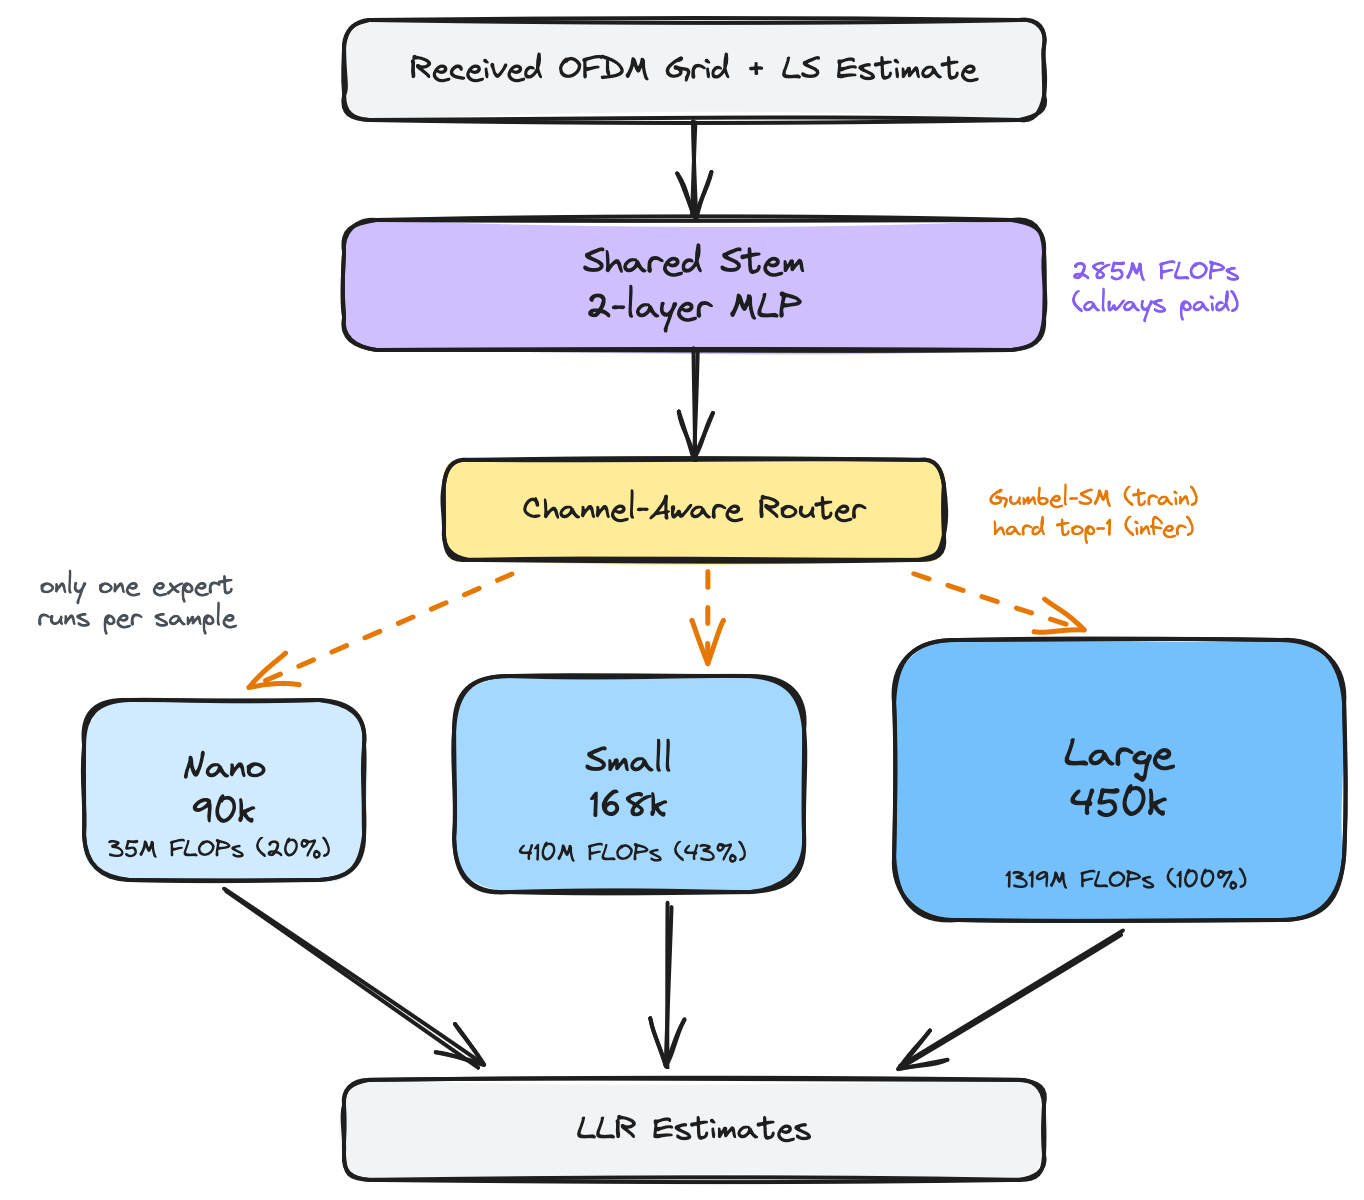
\includegraphics[width=0.95\linewidth]{figures/architecture.png}
  \vspace{0.3em}

  Three heterogeneous experts (\textbf{nano} 320\,M, \textbf{small} 695\,M, \textbf{large} 1604\,M FLOPs) plus a channel-aware router driven by stem features. Hard top-1 inference with no oracle SNR.
}

\block{Training recipe and validation}{
  Two failure modes during training: cold-start abandons \texttt{large}, full warm-start collapses to \texttt{large}. Eight literature-standard anti-collapse mechanisms (Switch aux $\times$ 4 weights, capacity $\times$ 4 weights) all fail.

  \vspace{0.5em}
  \textbf{Asymmetric warm-start with cold-\texttt{large}} works.
  \vspace{0.5em}

  \centering
\includegraphics[width=0.95\linewidth]{figures/expert_usage_asym_warm.pdf}
  \vspace{0.3em}

  Linear probes on stem features confirm channel-aware encoding: TDL-C SNR $R^2 = 0.93$, profile classification $77.9\,\%$. Replacing the router input with Gaussian noise raises BLER by \textbf{$+6.6$\,pp} and collapses routing.
}

%---------- RIGHT COLUMN ----------
\column{0.5}

\block{The training-scaffold finding}{
  \textbf{Per-expert success rate on the test set:}

  \vspace{0.3em}
  \centering
  \begin{tabular}{l c c}
    \toprule
    Expert & UMa success & TDL-C success \\
    \midrule
    nano  & $0.0\,\%$ & $0.0\,\%$ \\
    small & $0.0\,\%$ & $0.0\,\%$ \\
    \textbf{large} & $\mathbf{23.2\,\%}$ & $\mathbf{29.4\,\%}$ \\
    \bottomrule
  \end{tabular}
  \vspace{0.5em}

  \raggedright
  \textbf{Only \texttt{large} ever decodes a block.} The router sends work to \texttt{small} on samples where \emph{no} expert can decode. Forcing \texttt{large} on \texttt{small}'s samples gives BER $0.231$, BLER $1.000$ (large fails too). \texttt{small} matches \texttt{large}'s partial-decode quality at $43\,\%$ of the FLOPs.

  \vspace{0.5em}
  \textbf{Mode B: substitute \texttt{small} with a zero-output sink at inference.} BLER bit-identical, FLOPs drop $8.5$\,pp on the headline operating point. Generalises across the $\alpha$ sweep.

  \vspace{0.5em}
  {\centering
  \small
  \setlength{\tabcolsep}{4pt}
  \begin{tabular}{l c c c c}
    \toprule
     & BLER & BLER & FLOPs & FLOPs \\
    Checkpoint & base & Mode B & base & \textbf{Mode B} \\
    \midrule
    exp25 ($\alpha=10^{-3}$)              & 0.9063 & 0.9066 & 56.0\% & \textbf{46.7\%} \\
    \textbf{exp26} ($\alpha=2\cdot 10^{-3}$) & \textbf{0.9021} & \textbf{0.9021} & 55.8\% & \textbf{47.3\%} \\
    exp27 ($\alpha=5\cdot 10^{-3}$)        & 0.9107 & 0.9116 & 60.0\% & \textbf{41.9\%} \\
    \bottomrule
  \end{tabular}
  \par}
}

\block{Honest scope}{
  \raggedright
  Contribution scoped against the \textbf{dense neural} baseline. Compared to classical LMMSE LS-MRC (avg BLER $0.8997$ on $32\,768$ test samples per profile):
  \begin{itemize}
    \setlength\itemsep{0.3em}
    \item \textbf{TDL-C waterfall:} LMMSE wins by $2$--$3$\,dB SNR slack
    \item \textbf{UMa per-sample crosstab:} neural net $+64$ wins out of $32\,768$ ($n_{NN}{=}336$, $n_{LMMSE}{=}272$); NN-favoured subset has weaker MIMO geometry (spatial max eig $2.07$ vs $3.22$)
    \item \textbf{DeepMIMO ASU ray-traced OOD:} all neural decoders fail (BLER $\sim 0.99$); few-shot fine-tune did not recover
  \end{itemize}

  \vspace{0.5em}
  \textbf{What we claim.} A clean Pareto improvement vs the dense neural receiver, plus a training-scaffold interpretation: train with diverse experts for routing-policy gradient signal, prune the non-decoding middle expert at deployment.
}

\end{columns}

\block[bodyverticalshift=0mm]{}{
  \centering\footnotesize\itshape\color{darkgray}
  Every numerical claim verified against Weights \& Biases runs and analysis JSONs. Test set: $32\,768$ samples per profile. Code and run IDs in the project report.
}

\end{document}
